\section{Application Level Communications Interfaces}

This module provides a details on the higher application level communication interfaces used in the XMOS Motor Control Development Platform.
The figure below shows the main threads that are used.

\begin{figure}[h]
\begin{center}
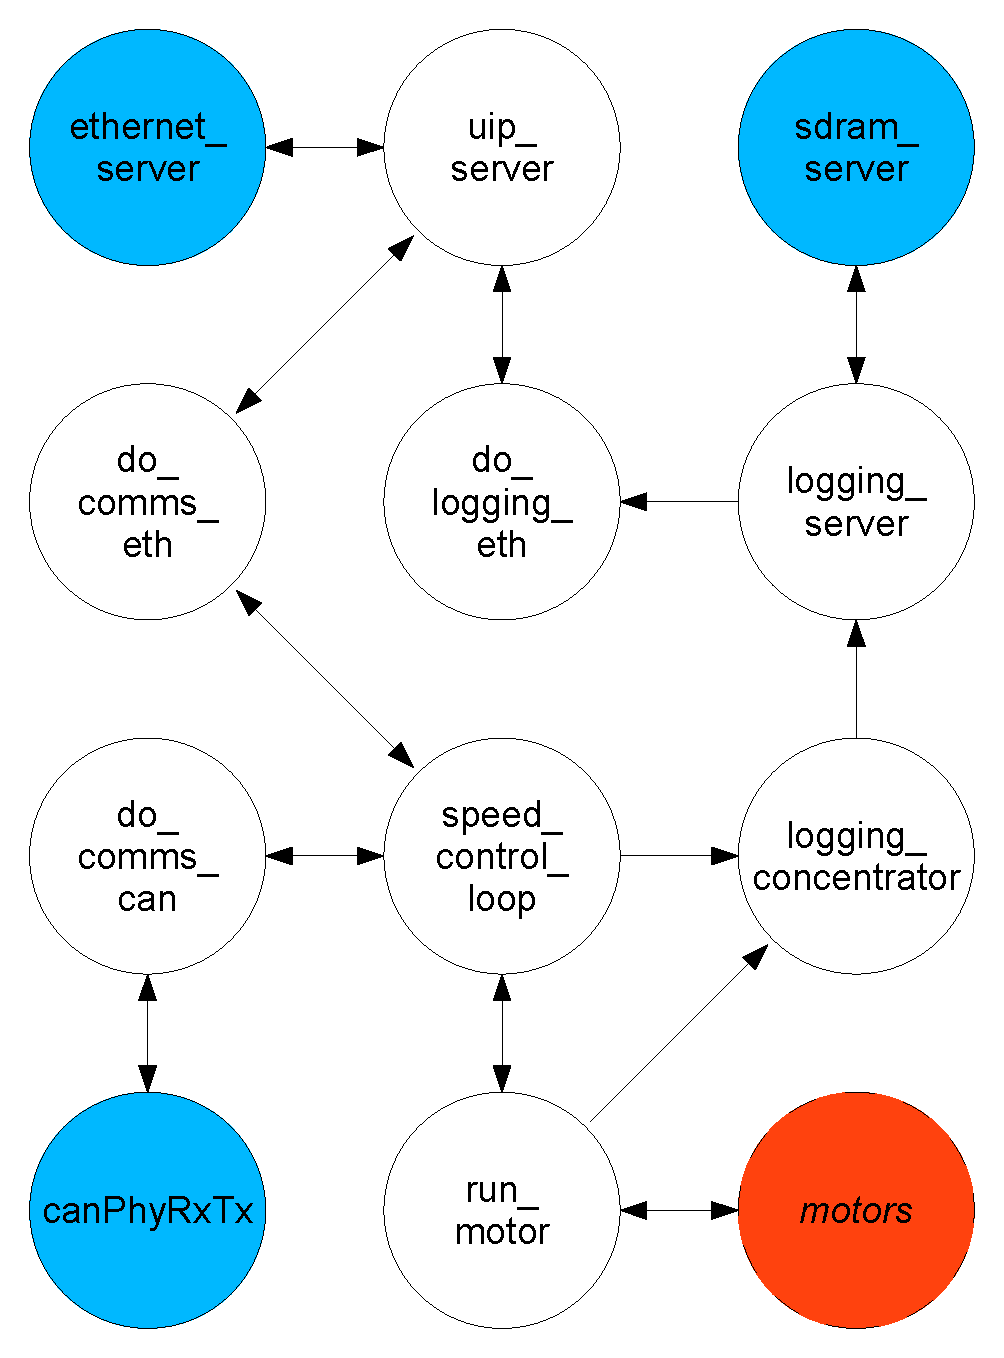
\includegraphics[height=0.6\textheight]{images/comms_threads}
\caption{Communications Thread Diagram}
\label{fig_comms_threads}
\end{center}
\end{figure}

The ethernet\_server and uip\_server threads are the Ethernet and TCP/IP interface, as detailed in the previous section.
The speed\_control\_loop and run\_motor threads are the outer and inner control loops for the motors.
The sdram\_server and canPhyRxTx are the SDRAM and CAN interfaces respectively, as previously discussed.


\subsection{do\_comms\_eth}

The thread do\_comms\_eth interfaces to the TCP/IP stack and provides a server interface on the TCP port defined by TCP\_CONTROL\_PORT (this is typically defined as 9595).

After configuring the TCP port and TCP/IP stack interface, the thread just sits in a \verb!while(1){}! loop processing TCP/IP events. 
The following actions are performed based on the event type:

\begin{itemize}
\item \verb!XTCP_NEW_CONNECTION! - Prints the IP address that the connection is from to the debug output.
\item \verb!XTCP_RECV_DATA! - Main processing function, described below.
\item \verb!XTCP_SENT_DATA! - Closes the send request by sending a 0 byte packet.
\item \verb!XTCP_REQUEST_DATA / XTCP_RESEND_DATA! - Sends the data generated during the \verb!XTCP_RECV_DATA! event to the client.
\item \verb!XTCP_CLOSED! - Closes the connection and prints the IP address that the connection was from to the debug output.
\end{itemize}

The main processing function, receives a packet from the client and processes it according to the criteria below: 

\begin{itemize}
\item if the packets starts "go" then this signals a new connection and nothing is done.
\item if the packets starts "set" then the next four little-endian ordered bytes are converted into the desired speed and sent to the speed\_control\_loop thread.
\item if the packets starts "speed" then the current and desired speeds from the speed\_control\_loop thread are placed in little-endian order into a packet of length 8 bytes and flagged to be returned to the client.
\item if the packets starts "stop" then the connection is closed.
\end{itemize}

The files for this thread are in:

\begin{itemize}
\item \verb!control_comms_eth.xc!
\item \verb!control_comms_eth.h!
\end{itemize}


\subsection{do\_logging\_eth}

The thread do\_logging\_eth interfaces to the TCP/IP stack and provides a server interface on the TCP port defined by TCP\_LOGGING\_PORT (this is typically defined as 9596).

After configuring the TCP port and the TCP/IP stack interface, the thread just sits in a \verb!while(1){}! loop processing TCP/IP events. 
The following actions are performed based on the event type:

\begin{itemize}
\item \verb!XTCP_NEW_CONNECTION! - Prints the IP address that the connection is from to the debug output.
\item \verb!XTCP_RECV_DATA! - Main processing function, described below.
\item \verb!XTCP_SENT_DATA! - Closes the send request by sending a 0 byte packet.
\item \verb!XTCP_REQUEST_DATA / XTCP_RESEND_DATA! - Sends the data generated during the \verb!XTCP_RECV_DATA! event to the client.
\item \verb!XTCP_CLOSED! - Closes the connection and prints the IP address that the connection was from to the debug output.
\end{itemize}

The main processing function, receives a packet from the client and processes it accordingly.
If the packets starts "go" then this signals a request for all the logging data in memory.
The thread then requests the data from the logging\_server thread in 4 byte chunks.
Once 1024 bytes has been received, the thread sends it to the client.

Alternatively, if the packet starts 'A', then this signals an acknowledgement from the host that the data was received and new data can be sent.
This is to force a packet to be generated, to mask the windows delayed ACK problem.
The thread then requests the next 1024 bytes of data from the logging\_server thread in 4 byte chunks, and sends it to the client.
No explicit command is given to signal the end of the data transmission.
The client will receive all data in the SDRAM, provided that every packet is acknowledged.

The files for this thread are in:

\begin{itemize}
\item \verb!logging_comms.xc!
\item \verb!logging_comms.h!
\end{itemize}


\subsection{logging\_server}

This thread controls the interface between the data coming for logging, the SDRAM and the Ethernet logging interface.

The basic operation of this thread, is that it sits in a \verb!while(1){}! loop using a select statement and a timer to log the data it receives from the logging\_concentrator to the SDRAM at 20kHz.
It can also receive requests from the do\_logging\_eth thread over a channel, which cause it to read the contents of all the SDRAM from the sdram\_server and send it back to the do\_logging\_eth thread.

The SDRAM is used as a circular buffer, with each data set (referred to as a record) being of SDRAM\_PACKET\_NWORDS in length.
For a length of 32 words (128 bytes) this gives 262144 records, which at 20kHz is 13.1 seconds of data being recorded.

Each record has a unique number as the first word, which is incremented by one for each record.
This allows the buffer to be de-circulated after it has been read.
When the data is read out, the entire contents of the SDRAM are sent over to the client from low to high memory addresses.
The client is then responsible for de-circulating the data.

The files for this thread are in:

\begin{itemize}
\item \verb!logging_if.xc!
\item \verb!logging_if.h!
\end{itemize}


\subsection{logging\_concentrator}

The function of the logging concentrator is to receive the data from each loop iteration of the outer and inner control loops for the motors.
It also decouples between the control loops and the logging\_server to prevent the pausing of one thread from disrupting the operation of the other.

The thread works by having a select sitting in a \verb!while(1){}! loop processing request on 3 different channels.
These channels are from the outer and inner control loops for the motors and the logging\_server respectively.
The data received from the control loops are placed into the relevant place in the current data packet buffer - this is constantly updated as new data comes in.
When the data is requested by the logging\_server the current packet buffer is streamed to this thread, along with a timestamp of when the request was made.
This means that there could be some jitter with the data, as well as some repeated or lost samples due to the data coming in and going out not being synchronised.

The files for this thread are in:

\begin{itemize}
\item \verb!logging_if.xc!
\item \verb!logging_if.h!
\end{itemize}


\subsection{do\_comms\_can}

This thread is similar in operation to the do\_comms\_eth thread, and provides the same interface to the speed\_control\_loop.

It works by configuring the CAN interface and then sitting in a \verb!while(1){}! loop receiving packets from the CAN interface.
Once the thread receives a packet from the client, it looks at the command type, and processes it accordingly.

\begin{itemize}
\item If command type (byte 2) equals 1, then this command sends the current speed and desired speed to the client.
\item If command type (byte 2) equals 2, then this command sets the desired speed from the data supplied in the packet.
\end{itemize}

The format of a received CAN packet is:

\begin{itemize}
\item 2 bytes - sender address - used to address the return packet if required.
\item 1 byte - command type 
\item 4 bytes - desired speed in big-endian order if command equals 2.
\end{itemize}

The format of a transmitted CAN packet is:

\begin{itemize}
\item 4 bytes - current speed in big-endian order.
\item 4 bytes - desired speed in big-endian order.
\end{itemize}

The files for this thread are in:

\begin{itemize}
\item \verb!control_comms_can.xc!
\item \verb!control_comms_can.h!
\end{itemize}


